\documentclass[11pt]{article}
\usepackage[margin=1in]{geometry}
\usepackage{graphicx}
\usepackage{amsmath}
\usepackage{booktabs}
\usepackage{hyperref}
\usepackage{parskip}
\usepackage{float}
\widowpenalty=10000
\clubpenalty=10000
\hypersetup{colorlinks=true, urlcolor=blue, linkcolor=black}
\graphicspath{{figures/}}
\title{Historical Rainfall across Singapore (2017--2024):\\ Weather-Pattern Analysis and 30-Minute Exceedance Prediction with Apache Spark}
\author{}
\date{}
\begin{document}
\maketitle

\section{Introduction}

Rainfall in Singapore varies both seasonally and over the course of a day. This project examines those patterns using five-minute rainfall readings from 91 stations between 2017 and 2024, obtained from \href{https://data.gov.sg/collections/2279/view}{data.gov.sg collection 2279}. It then uses the same data to estimate the probability that a station will receive more than a specified amount of rain in the next 30 minutes.

The work is organised into two tasks. Task 1 describes rainfall frequency, intensity, annual totals, and the daily cycle. Task 2 trains and evaluates a classifier that takes the rainfall threshold as an input, alongside station, time, and recent rainfall information. Apache Spark is used for data preparation, analysis, and model training.

The report follows the main decisions from data cleaning through to evaluation. Reproduction instructions are provided in \texttt{README.md}.

\section{Data preparation and computing environment}

\subsection{Execution environment}

Data preparation, exploratory analysis, and sampled model training were carried out on an Apple M4 Pro with 14 cores and 48\,GB RAM, running macOS 27. The local software environment used Spark 3.5.3 through PySpark, Python 3.11, and Eclipse Temurin JDK 11. Python dependencies were managed with \texttt{uv}, and the JDK was extracted into the project directory.

Full-data training ran on Google Cloud Dataproc using image \texttt{2.3-debian12}, with Spark 3.5.3, Scala 2.12, and JDK 11. The cluster had one master and four workers, all \texttt{n4-standard-4} instances with four vCPUs and Hyperdisk Balanced boot disks. The same training script was used in both environments. All cloud resources were deleted after the run.

\subsection{Cleaning timestamps and selecting stations}

Each observation is identified by its station and timestamp and records rainfall for a five-minute slot. The source CSVs include Singapore's UTC+8 offset. Spark preserves the time of each observation when converting the data to Parquet. For example, a CSV timestamp of \texttt{08:00+08:00} represents the same moment as 00:00 UTC and appears as 08:00 when read in Singapore time. The analysis uses these local times to examine seasonal and daily rainfall patterns.

The 2017 readings also occur one second before the expected five-minute boundary, for example at 08:04:59 rather than 08:05:00. Cleaning adds one second and truncates to the minute. Duplicate station--timestamp pairs created at the boundary were removed, affecting approximately 58 rows.

Station coverage varies across the eight years. Stations were retained if they had at least 1{,}000 readings, at least 90\% completeness between their first and last observations, and some nonzero rainfall. Measuring completeness over each station's own recorded lifespan allowed stations introduced in mid-2020 to remain in the analysis when their coverage during that period was adequate.

These checks retained 67 of the 91 stations. One excluded station, S24B, had approximately 33{,}000 readings but never recorded rain. Every other station recorded rain during the same period, supporting its exclusion as a suspected stuck sensor. Figure~\ref{fig:map} shows the retained stations.

\begin{figure}[H]
  \centering
  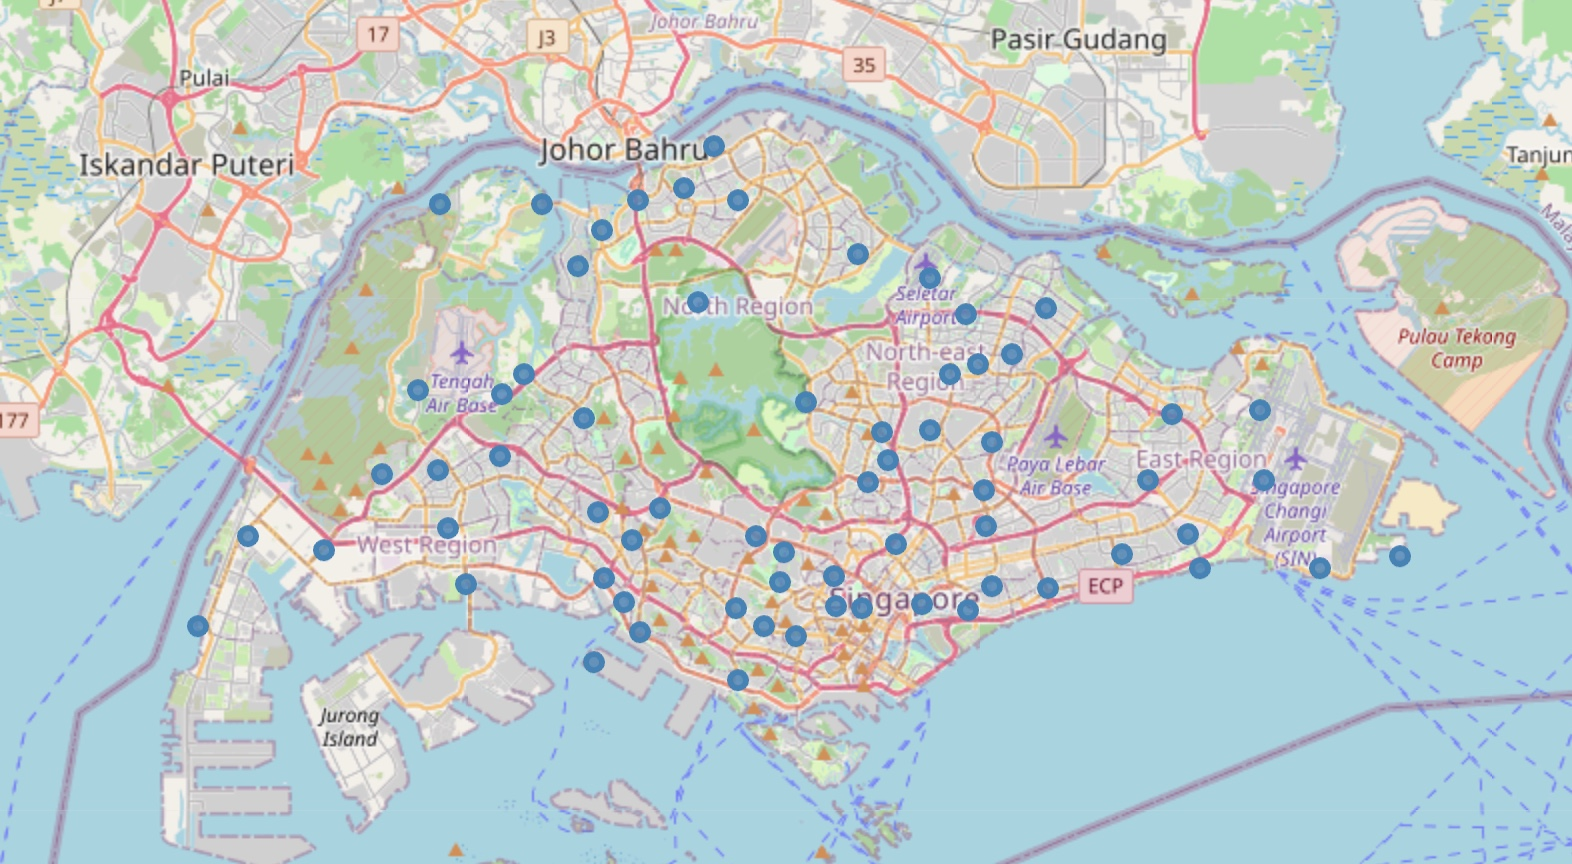
\includegraphics[width=0.9\linewidth]{station_map2.jpeg}
  \caption{Locations of the 67 retained rainfall stations.}
  \label{fig:map}
\end{figure}

About 97\% of five-minute readings are zero, and the smallest nonzero reading is approximately 0.2\,mm, consistent with the gauge resolution. Both the large number of dry slots and the discrete measurement scale matter for the prediction task. In particular, a strict exceedance of 0.2\,mm excludes an accumulation of exactly 0.2\,mm; it is therefore different from detecting any rain.

\section{Task 1: Rainfall patterns}

The changing station roster requires care when combining observations. For monthly frequency and annual totals, readings were first aggregated across the stations reporting in each five-minute slot, then over time. This gives each observed slot equal weight. It also avoids an earlier problem in which partial station-years were summed and treated as complete annual totals. The estimates still depend on the locations of the stations reporting at each time.

\subsection{Seasonal frequency and intensity}

Rainfall frequency was calculated as the fraction of reporting stations with nonzero rain in each five-minute slot, averaged within each month and year. Figure~\ref{fig:freq} shows the mean across 2017--2024 together with the variation between years. Rain was most frequent from November to January, during the Northeast Monsoon. The mid-year Southwest Monsoon did not show a similarly distinct frequency peak in this dataset.

\begin{figure}[H]
  \centering
  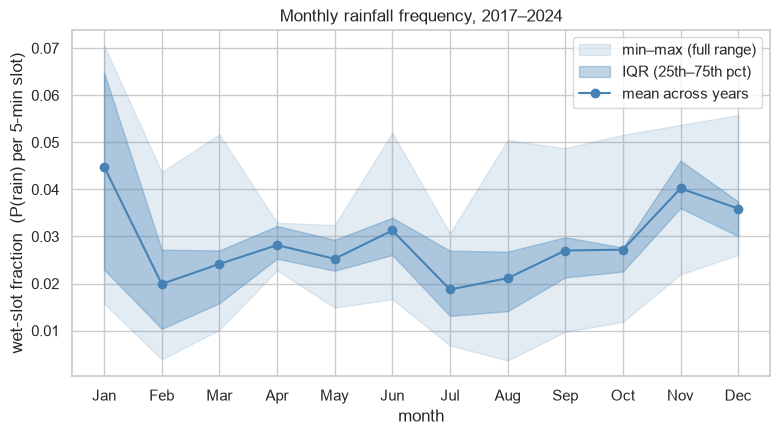
\includegraphics[width=0.8\linewidth]{plotA.png}
  \caption{Monthly rainfall frequency, averaged across 2017--2024. Bands show the interquartile range and full range across years.}
  \label{fig:freq}
\end{figure}

Frequency alone does not describe how much rain falls when it rains. To examine intensity, rainfall was averaged across the wet stations in each five-minute slot, then across wet slots within each month and year. This produces a different seasonal pattern (Figure~\ref{fig:int}): January had the lowest intensity, while March--April had the highest. The months with the most frequent rain therefore did not have the heaviest rain per wet slot. Using separate measures makes this distinction visible.

\begin{figure}[H]
  \centering
  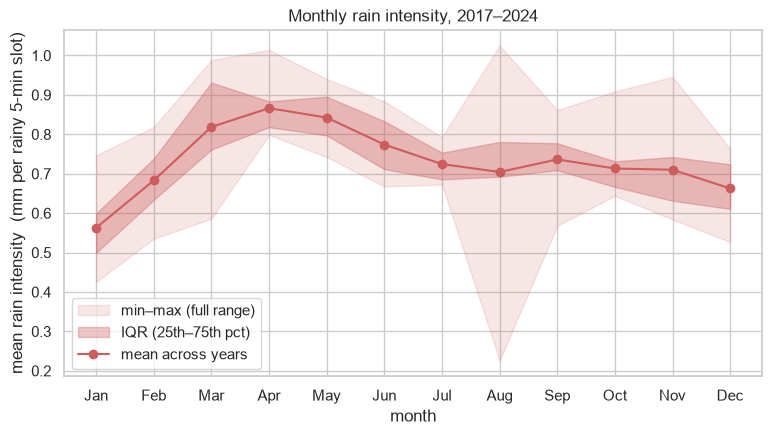
\includegraphics[width=0.8\linewidth]{plotB.png}
  \caption{Monthly rainfall intensity: mean rainfall at wet stations per five-minute slot, averaged over wet slots and then across years.}
  \label{fig:int}
\end{figure}

\subsection{Variation between years}

Annual totals were obtained by summing the station-average rainfall in each five-minute slot. Totals ranged from approximately 1{,}700\,mm in 2019 to 2{,}900\,mm in 2021--2022 (Figure~\ref{fig:annual}). There was substantial variation between years, without a consistent increase or decrease. Eight years of data are insufficient to establish a long-term trend, so no trend line was fitted.

\begin{figure}[H]
  \centering
  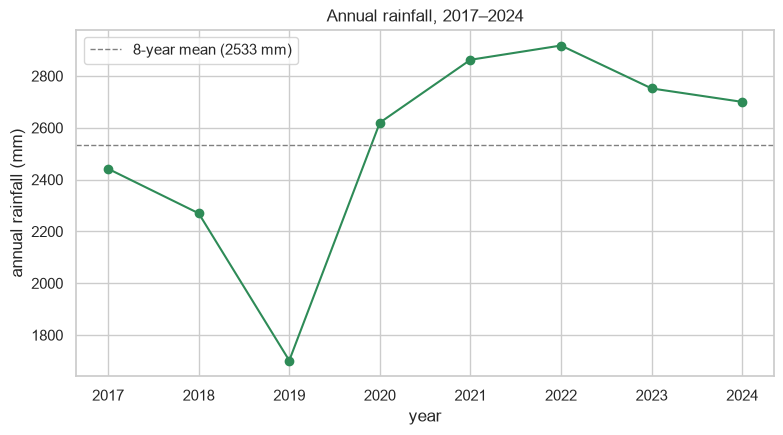
\includegraphics[width=0.8\linewidth]{plotC.png}
  \caption{Annual rainfall totals for 2017--2024, calculated from the five-minute station averages.}
  \label{fig:annual}
\end{figure}

\subsection{The daily cycle}

The hourly analysis used a different unit: the station-hour. For each station, date, and hour, an hour was marked as wet if any available five-minute reading recorded rain. These indicators were then averaged by local hour across all observed station-hours.

Rain was most common around 15:00 (Figure~\ref{fig:diurnal}). Approximately 16\% of station-hours at that time recorded rain, compared with about 3.5\% overnight, a ratio of roughly 4.5. This clear daily cycle provides a reason to include time of day in the prediction model, alongside seasonal information. It also illustrates why the timezone check mattered: UTC hours would have placed the peak around 07:00.

\begin{figure}[H]
  \centering
  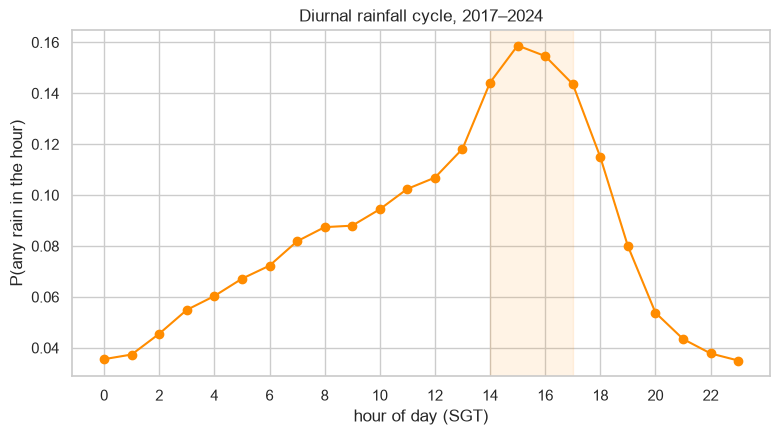
\includegraphics[width=0.8\linewidth]{plotD.png}
  \caption{Fraction of observed station-hours recording any rain, by hour of day in Singapore time.}
  \label{fig:diurnal}
\end{figure}

\section{Task 2: Predicting 30-minute exceedance}

\subsection{Target and features}

The prediction task asks whether rainfall at a station will exceed a threshold $X$ in the next 30 minutes. At time $t$, the target accumulation is the sum of the next six five-minute readings, from $t+5$ to $t+30$. The binary label is 1 when that sum exceeds $X$, and 0 otherwise. Labels were constructed only when all six future slots were present and contained non-null, non-negative readings. Incomplete windows were excluded rather than treated as dry periods.

To make the threshold a model input, each station--time observation was replicated over a grid of 0.2, 1, 2, 5, and 10\,mm, selected from the accumulation distribution. The label was recalculated for each threshold, and a single classifier was trained with the threshold as a feature. This gives an exceedance probability directly without fitting a separate classifier for each threshold. Quantile regression was considered, but obtaining exceedance probabilities would require estimating and interpolating multiple quantiles. Although the classifier can accept other threshold values, performance was evaluated only at the five training thresholds.

\newpage
The remaining features describe the station, the time, and rainfall observed at or before $t$:

\begin{itemize}
  \item The station's readings at $t$, $t-5$, $t-10$, $t-15$, and $t-20$ minutes. Lags were joined by timestamp so that a missing slot remained missing, rather than being replaced by an older reading through a row-offset lookup.
  \item Island-wide conditions at $t$: the fraction of reporting stations recording rain, mean and maximum rainfall, rainfall standard deviation, and the number of reporting stations.
  \item Sine and cosine encodings of minute-of-day and day-of-year. Minute-of-day distinguishes the twelve five-minute slots within an hour.
  \item Station identifier, latitude, and longitude.
\end{itemize}

The feature set was kept small. Rolling averages were omitted because recent readings were already available to the tree model, and month was omitted because day-of-year represented the seasonal cycle. Missing values were preserved in the feature table and handled during training.

\subsection{Choosing and implementing the model}

LightGBM through SynapseML was the initial choice, but attempts to run it on Dataproc encountered several problems. Cloud NAT resolved package downloads on internal-IP nodes. Barrier execution addressed a driver--worker socket handshake failure and required Spark dynamic allocation to be disabled. After these changes, a single-node run exhausted memory, and a four-worker run failed with a segmentation fault in LightGBM's native library, recorded in the YARN container logs. The native library also failed to load in the local Apple Silicon environment.

The model was therefore changed to Spark MLlib's \texttt{GBTClassifier}. Its JVM implementation avoided the native-library dependency and allowed the same script to run locally and on Dataproc. Missing lag readings and spatial standard deviations were filled with $-1$ before training. Since observed values for these features are non-negative, this sentinel distinguishes missing data from zero.

A further requirement is that exceedance probability must not rise as the threshold increases. GBT does not enforce this during training, so the predictions were adjusted afterwards. For each station--time observation, thresholds were ordered from largest to smallest and each probability was replaced by the running maximum. The adjusted probabilities were used for evaluation.

The saved pipeline contains a \texttt{StringIndexer} for station identifiers, a \texttt{VectorAssembler}, and the GBT classifier. Latitude and longitude provide additional location information. The \texttt{maxBins} setting was 128, above the number of retained stations.

\subsection{Training and evaluation}

Hyperparameters were selected using 2023 as a validation year and earlier years for training. Among the configurations tested, depth 3 underfit and depth 7 overfit, while the learning-rate configurations gave similar validation scores. The selected settings were \texttt{maxDepth=5}, \texttt{maxIter=60}, and \texttt{stepSize=0.1}, balancing validation performance and training cost.

The final models were trained on data through 2023 and tested on 2024. A 30-minute gap before the test period prevented training labels from using rainfall in the test year. Two training runs were compared: a 10\% sample trained locally, and the full dataset trained on Dataproc. Both used the full 2024 test set.

Metrics were calculated separately for each threshold because the positive rate varies from approximately 4.9\% at 0.2\,mm to 0.4\% at 10\,mm. PR-AUC was the primary metric, with ROC-AUC reported alongside it. F1, precision, and recall were calculated at a probability cutoff of 0.5.

\begin{table}[H]
  \centering
  \caption{PR-AUC on the 2024 test set: 10\% local sample versus full-data training (approximately 160 million threshold-expanded rows). The two test sets both cover 2024 but are not identical (5{,}562{,}959 rows locally vs 5{,}557{,}581 in the cloud); see the timezone note below. The Difference column is computed from the unrounded PR-AUC values.}
  \label{tab:prauc}
  \begin{tabular}{lccc}
    \toprule
    Threshold & PR-AUC (10\% sample) & PR-AUC (full) & Difference \\
    \midrule
    $>$0.2\,mm & 0.755 & 0.756 & $+0.002$ \\
    $>$1\,mm   & 0.674 & 0.675 & $+0.001$ \\
    $>$2\,mm   & 0.594 & 0.600 & $+0.006$ \\
    $>$5\,mm   & 0.474 & 0.476 & $+0.002$ \\
    $>$10\,mm  & 0.364 & 0.367 & $+0.003$ \\
    \bottomrule
  \end{tabular}
\end{table}

\begin{table}[H]
  \centering
  \caption{Full-data model: all metrics on the 2024 test set, per threshold. PR-AUC and ROC-AUC use the predicted probabilities; F1, precision, and recall use a 0.5 cutoff.}
  \label{tab:fullmetrics}
  \begin{tabular}{lccccc}
    \toprule
    Threshold & PR-AUC & ROC-AUC & F1 & Precision & Recall \\
    \midrule
    $>$0.2\,mm & 0.756 & 0.952 & 0.666 & 0.813 & 0.563 \\
    $>$1\,mm   & 0.675 & 0.952 & 0.593 & 0.798 & 0.471 \\
    $>$2\,mm   & 0.600 & 0.963 & 0.529 & 0.741 & 0.412 \\
    $>$5\,mm   & 0.476 & 0.964 & 0.395 & 0.715 & 0.273 \\
    $>$10\,mm  & 0.367 & 0.974 & 0.293 & 0.640 & 0.190 \\
    \bottomrule
  \end{tabular}
\end{table}

PR-AUC was well above the positive base rate at every threshold (Table~\ref{tab:fullmetrics}). For the full-data model it was 0.756 at 0.2\,mm and 0.367 at 10\,mm, against positive rates of approximately 0.049 and 0.004 respectively. ROC-AUC ranged from 0.95 to 0.97. PR-AUC decreased at the higher thresholds, where heavy-rain events were rarer. At the 0.5 cutoff, precision was relatively high but recall was low, particularly for heavy rain; lowering the cutoff could increase recall at the expense of precision.

The full-data model improved PR-AUC by at most about 0.006 over the sampled model, and by only 0.001--0.003 at most thresholds (Table~\ref{tab:prauc}). Training on the 10\% sample therefore gave essentially the same performance at a lower computational cost. Two caveats make this an indicative rather than exact comparison. First, the sampled run used 40 boosting iterations against the full run's 60. Second, the two runs used year-boundary cutoffs eight hours apart: the training script created the \texttt{2024-01-01} cutoff as a timezone-naive timestamp, which PySpark converted using the Python driver process's local timezone: Singapore time locally (test from 00:00 SGT) and UTC on Dataproc (test from 08:00 SGT). The cloud test set therefore omits the first eight hours of 2024 --- 5{,}378 observations per threshold ($\sim$0.097\% of the local test set), containing 49, 6, 4, 0, and 0 positive events at the five thresholds. Given the small proportion of observations and positive events affected, the impact on the evaluation metrics is expected to be small, but has not been quantified by rescoring both models on an identical test set. The training and tuning scripts now use explicitly timezone-aware Singapore calendar-year boundaries as well as the Singapore session timezone; the saved models predate this correction. This does not establish that further data would never help: repeated samples and evaluation on other years would be needed to assess how consistently the two approaches perform.

Full-data training was memory-bound and spilled to disk on the four-worker cluster. It took more than ten times as long as the sampled local run, although the different hardware environments limit a direct timing comparison. Before another full-data run, a higher-memory cluster or revised partitioning strategy could be investigated.

\section{Using the model and interpreting its limits}

The task asks for a probability given a station, a prediction time, and a threshold. The script \texttt{scripts/predict.py} provides exactly that interface: it takes the three inputs, derives the model's features from the cleaned rainfall data, and returns the exceedance probability. The rainfall data is required because features such as the reading 15 minutes earlier and the island-wide context are functions of the station and time rather than user inputs.

The model is saved as a Spark ML \texttt{PipelineModel} directory and must be loaded in a Spark session. Missing-value filling and the monotonic adjustment lie outside the saved pipeline. The following code fills missing features and obtains the raw predictions; it does not yet apply the monotonic adjustment:

\begin{verbatim}
from pyspark.ml import PipelineModel

missing_cols = ["rain_t5", "rain_t10", "rain_t15", "rain_t20", "isl_std"]
features_df = features_df.fillna({c: -1.0 for c in missing_cols})
model = PipelineModel.load("models/run-001/model")
preds = model.transform(features_df)
\end{verbatim}

In single mode, \texttt{predict.py} scores the five training thresholds plus the requested threshold if it is not already on the grid. It then takes a running maximum of the raw probabilities in descending threshold order and returns the adjusted probability for the requested threshold. This ensures that the probabilities do not increase across the thresholds scored together. Batch mode applies the same adjustment to the threshold rows present for each station--time observation, although sampling can leave an incomplete grid. During test-set evaluation, \texttt{scripts/train.py} applies missing-value filling and the adjustment across the full five-threshold grid.

The evaluation shows that the model can distinguish exceedance events in the 2024 data, but several questions remain before practical use. First, probability calibration was not assessed. A reliability curve and Brier score would help determine whether predicted probabilities agree with observed event frequencies. Second, the 0.5 decision cutoff was not chosen for a particular application. A cutoff should be selected on validation data according to the costs of missed events and false alarms.

Evaluation was also limited to one held-out year. The test set contains approximately 28 million threshold-expanded rows and covers all seasons, but its size does not establish performance across years. Rolling-origin evaluation would help assess this variation and the reliability of the sample-training comparison.

Finally, readings are published approximately 10--15 minutes after their timestamp. The experiments use the observation timestamp as the prediction reference. A live system would need to construct features from readings that had actually arrived by the prediction time, which could change its performance.

\section{Conclusion}

The rainfall analysis found distinct seasonal patterns in frequency and intensity, substantial variation in annual totals, and a clear afternoon peak in the likelihood of rain. Accurate local timestamps and careful treatment of station coverage were necessary to describe these patterns correctly.

For 30-minute exceedance prediction, Spark MLlib GBT provided a workable model in both local and cloud environments after the LightGBM attempts failed. Full-data training gave only a small improvement over the 10\% sample in the 2024 evaluation. The next steps would be to test across more years, assess probability calibration, and account for reporting delay in a realistic prediction setup.

\section{AI usage declaration}

Anthropic's Claude, through the Claude Code CLI, assisted with code implementation and with setting up and troubleshooting Google Cloud Dataproc. It also assisted with the clarity and phrasing of this report. All instructions, analytical approaches, modelling decisions, and overall project direction were provided by the author. AI-generated code was reviewed, tested, and executed by the author. The reported results are from actual experimental runs and the author's analysis.

\end{document}
